\documentclass[tikz,border=2pt]{standalone}
\usepackage{amsmath}
\usetikzlibrary{arrows.meta}
\begin{document}
% English auction with private values 40, 55, 70 and the dominant strategy "quit at your value":
% bidder 1 drops out at 40, bidder 2 at 55; bidder 3 wins at price 55 (the second-highest value)
% and keeps 70 - 55 = 15.
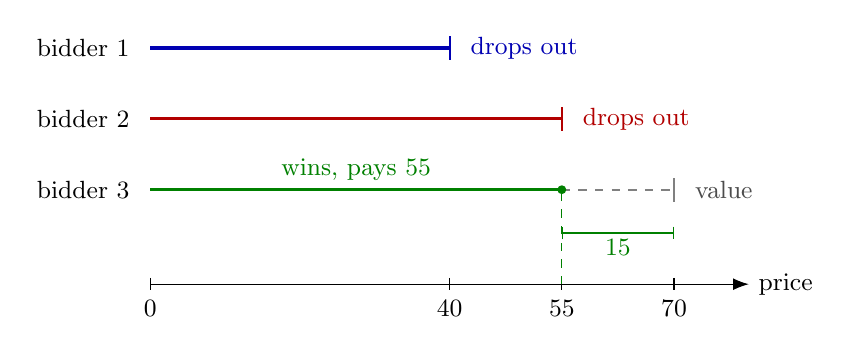
\begin{tikzpicture}[font=\small, >={Latex[length=2mm]}, x=0.095cm, y=1cm]
  % price axis
  \draw[->] (0,0) -- (80,0) node[anchor=west] {price};
  \foreach \p in {0,40,55,70}
    \draw (\p,0.08) -- (\p,-0.08) node[anchor=north] {$\p$};
  % bidders' active intervals
  \draw[blue!70!black, very thick] (0,3.0) -- (40,3.0);
  \draw[blue!70!black, thick] (40,2.85) -- (40,3.15);
  \node[blue!70!black, anchor=west] at (41.5,3.0) {drops out};
  \draw[red!70!black, very thick] (0,2.1) -- (55,2.1);
  \draw[red!70!black, thick] (55,1.95) -- (55,2.25);
  \node[red!70!black, anchor=west] at (56.5,2.1) {drops out};
  \draw[green!50!black, very thick] (0,1.2) -- (55,1.2);
  \draw[gray, thick, dashed] (55,1.2) -- (70,1.2);
  \fill[green!50!black] (55,1.2) circle (1.6pt);
  \draw[gray, thick] (70,1.05) -- (70,1.35);
  \node[gray!60!black, anchor=west] at (71.5,1.2) {value};
  \node[anchor=east] at (-1.5,3.0) {bidder 1};
  \node[anchor=east] at (-1.5,2.1) {bidder 2};
  \node[anchor=east] at (-1.5,1.2) {bidder 3};
  % winner's surplus
  \draw[green!50!black, thin, |-|] (55,0.65) -- node[anchor=north, fill=white, inner sep=1pt, yshift=-1pt] {$15$} (70,0.65);
  % auction ends
  \draw[green!50!black, thin, dashed] (55,0) -- (55,1.2);
  \node[green!50!black, anchor=south] at (27.5,1.2) {wins, pays $55$};
\end{tikzpicture}
\end{document}
